\documentclass{article}
\usepackage[utf8]{inputenc}
\usepackage{amsmath}
\usepackage{amssymb}
\usepackage{amsfonts}
\usepackage{graphicx}
\usepackage{tikz}
\usetikzlibrary{angles,fit,arrows,calc,math,matrix,intersections,through,backgrounds,cd}
\usepackage{pgfplots}
\pgfplotsset{compat=1.18}
\usepackage{geometry}
\geometry{a4paper, margin=1in}
\usepackage{booktabs} % For professional looking tables

\title{Systematic Study of $K$ Values in Global Arithmetic Torsion for the $4_1$ Knot}
\author{Manus}
\date{\today}

\begin{document}
\maketitle

\section{Introduction}
This document presents a systematic study of the integer $K$ that appears in the global arithmetic torsion formula, $\mathcal{T}(S) = \Delta(t)(t^K-1)$, specifically for the figure-eight knot ($4_1$). This investigation aims to understand the conditions under which $K$ takes certain values by analyzing various paths (relators) in the knot group $G(4_1)$, using data provided in the `aeg-paper` repository.

The figure-eight knot, denoted as $4_1$, is a prime, alternating knot with a crossing number of four. It is the simplest hyperbolic knot.

\begin{figure}[h!]
    \centering
    % Assuming knot_4_1.tex is in a figures subdirectory relative to this file
    \documentclass{standalone}
\usepackage{amsthm}
\usepackage{amssymb}
\usepackage{amsfonts}
\usepackage{amsmath}
\usepackage{mathtools}

\usepackage{pgf}
\usepgflibrary{fpu}
\usepackage{pgfplots}
\usepackage{tikz}
\usetikzlibrary{angles,fit,arrows,calc,math,matrix,intersections,through,backgrounds,cd}
\usepackage{tkz-euclide}
\usepackage{tkz-graph}
\usepackage{graphicx}
\pgfplotsset{compat=1.18}

\begin{document}

        \tikzmath{
                \one = 1;
                \base = 2.618033988749;
                \offset = 15.8888888;
                \valofpi = 3.1415926;
                \anglei = 3.1415926;
                \angleo = 3.1415926;
        }

        \begin{tikzpicture}[scale=1.0]
                % 1. 绘制坐标轴
                \draw[black, line width=0.6pt, ->]
                (\offset,0) to[out=90,in=270] (\offset,15.5)
                node [anchor=south] {y};

                \draw[black, line width=0.6pt, ->]
                (-7.5,0) to[out=0,in=180] (18,0)
                node [anchor=west] {x};

                % 2. 绘制 x 和 y 坐标轴刻度
                \foreach \x in {-25,...,2} {
                        \node [anchor=north] at (\x/9*8 + \offset, 0) {\x};
                }
                \foreach \y in {1,...,17} {
                        \node [anchor=-135] at (18, \y/9*8) {\y};
                }

                % 3. 浅灰色水平网格线
                \foreach \t in {17,...,1} {
                        \draw [lightgray, line width=0.6pt]
                        (-7.5,\t/9*8)
                        to[out=0,in=180]
                        (18,\t/9*8);
                }

                % 4. 浅灰色竖直网格线
                \foreach \t in {-26,...,2} {
                        \draw [lightgray, line width=0.6pt]
                        (\t/9*8 + \offset, 0)
                        to[out=90,in=270]
                        (\t/9*8 + \offset, 15.5);
                }




        \end{tikzpicture}
\end{document}
 
    \caption{The Figure-Eight Knot ($4_1$).}
    \label{fig:knot_4_1}
\end{figure}

\section{Background: Global Arithmetic Torsion}
The concept of global arithmetic torsion is given by the expression $\mathcal{T}(S) = \Delta(t)(t^K-1)$. Here, $\Delta(t)$ is the Alexander polynomial of the knot ($t^2 - 3t + 1$ for the $4_1$ knot), $t$ is a parameter, and $K$ is an integer that depends on the chosen path $S$ (a relator) within the knot group $G(4_1)$.

\section{Analysis of $K$ Values from Provided Data}

Data for the knot $4_1$ is available in the `knots/results.tex` file within the `aeg-paper` repository. The relevant section for knot $4_1$ is presented and analyzed below.

\subsection{Data from \texttt{results.tex} for Knot $4_1$}

\noindent The provided data indicates the following for knot $4_1$:

\begin{itemize}
    \item Alexander polynomial: $\Delta(a) = a^2 - 3a + 1$.
    \item Cyclotomic polynomials: $\Phi_1(a) = a-1$, $\Phi_2(a) = a+1$.
    \item Path-dependent terms: $p(a) = \nu(S_R)(0,a)$ and $q(a) = \nu(S_{R_{\text{rev}}})(0,a)$.
    \item Torsion: $\tau(a) = p(a) - q(a)$.
\end{itemize}

\begin{table}[h!]
\centering
\caption{Summary of Arithmetic Torsion Analysis for Knot $4_1$ (Unified Mapping, from \texttt{results.tex}).}
\label{tab:knot41_data}
\scriptsize
\begin{tabular}{@{}p{3.2cm} p{2.0cm} p{2.0cm} p{2.5cm} p{3.3cm} p{3.3cm}@{}}
\toprule
\textbf{Relator(s) Used} & \textbf{$p(a)$} & \textbf{$q(a)$} & \textbf{Torsion $\tau(a) = p(a) - q(a)$} & \textbf{Torsion Factors} & \textbf{Notes} ($k_p, k_q, \sigma_{\text{eff}}$; Cyclot. Factors) \\
\midrule
\texttt{aaBAbbbAB}, \texttt{abbbaBAAB} & $-\Delta(a)$ & $-\frac{\Delta(a)}{a^2}$ & $\frac{-\Delta(a)(a^2-1)}{a^2}$ & $\frac{-\Delta(a) \Phi_1(a) \Phi_2(a)}{a^2}$ & $k_p=0, k_q=2, \sigma_{\text{eff}}=-1$; Cyclot. $\Phi_1\Phi_2$ \\
\addlinespace
\texttt{aBAABabbb}, \texttt{bbbABaaBA}, \texttt{bbbaBAABa} & $-\frac{\Delta(a)}{a}$ & $-\frac{\Delta(a)}{a}$ & $0$ & $0$ & $k_p=1, k_q=1, p(a)=q(a)$; No cyclot. part \\
\bottomrule
\end{tabular}
\end{table}

\subsection{Derivation of $K$}
We use the formula $\mathcal{T}(S) = \Delta(a)(a^K-1)$. The term $\mathcal{T}(S)$ corresponds to the "Torsion $\tau(a)" $ column from Table \ref{tab:knot41_data} (with the variable $t$ replaced by $a$ for consistency with the table notation).
Thus, $a^K-1 = \frac{\tau(a)}{\Delta(a)}$.

\subsubsection{Case 1: Relators \texttt{aaBAbbbAB}, \texttt{abbbaBAAB}}
From Table \ref{tab:knot41_data}, for these relators:
\[ \tau(a) = \frac{-\Delta(a)(a^2-1)}{a^2} \]
Assuming $\Delta(a) \neq 0$, we substitute this into the equation for $a^K-1$:
\[ a^K-1 = \frac{1}{\Delta(a)} \left( \frac{-\Delta(a)(a^2-1)}{a^2} \right) = \frac{-(a^2-1)}{a^2} = \frac{1-a^2}{a^2} \]
Therefore,
\[ a^K = 1 + \frac{1-a^2}{a^2} = \frac{a^2 + 1 - a^2}{a^2} = \frac{1}{a^2} = a^{-2} \]
This implies that for these relators, $K = -2$.

The notes in the table ($k_p=0, k_q=2, \sigma_{\text{eff}}=-1$) provide parameters related to the specific computational framework used to derive $p(a)$ and $q(a)$. The derived $K=-2$ is a direct consequence of the torsion formula and the reported $\tau(a)$.

\subsubsection{Case 2: Relators \texttt{aBAABabbb}, \texttt{bbbABaaBA}, \texttt{bbbaBAABa}}
From Table \ref{tab:knot41_data}, for these relators:
\[ \tau(a) = 0 \]
Assuming $\Delta(a) \neq 0$, we have:
\[ a^K-1 = \frac{0}{\Delta(a)} = 0 \]
This implies $a^K = 1$. If $a$ is not a root of unity, then $K=0$.
This case is of particular interest as it signifies a vanishing component of the arithmetic torsion. The notes confirm $p(a)=q(a)$ for these paths, leading directly to $\tau(a)=0$.

\section{Discussion of Path Properties and $K$ Values}

The analysis reveals two distinct $K$ values for the provided sets of relators for the $4_1$ knot:
\begin{itemize}
    \item $K = -2$ for relators like \texttt{aaBAbbbAB}.
    \item $K = 0$ for relators like \texttt{aBAABabbb}.
\end{itemize}

Further investigation would involve:
\begin{enumerate}
    \item **Algebraic Structure of Relators:** Analyzing the word structure of these relators in the generators of $G(4_1)$ (e.g., Wirtinger presentation or other common presentations like $\langle x,y \mid xyx^{-1}yxy^{-1}x^{-1}y^{-1} \rangle = 1$) to identify features correlating with $K=-2$ versus $K=0$. This could involve looking at exponent sums, subword patterns, or relationships to specific group operations.
    \item **Geometric Interpretation in (U,V) Space:** Visualizing these paths in the $(U,V)$ reference space, as conceptualized in related research questions. The geometric properties (net displacement, enclosed area, winding numbers) of paths leading to $K=-2$ versus $K=0$ could reveal underlying geometric reasons for the different $K$ values.
    \begin{figure}[h!]
        \centering
        % Assuming uv_path_example.tex is in a figures subdirectory relative to this file
        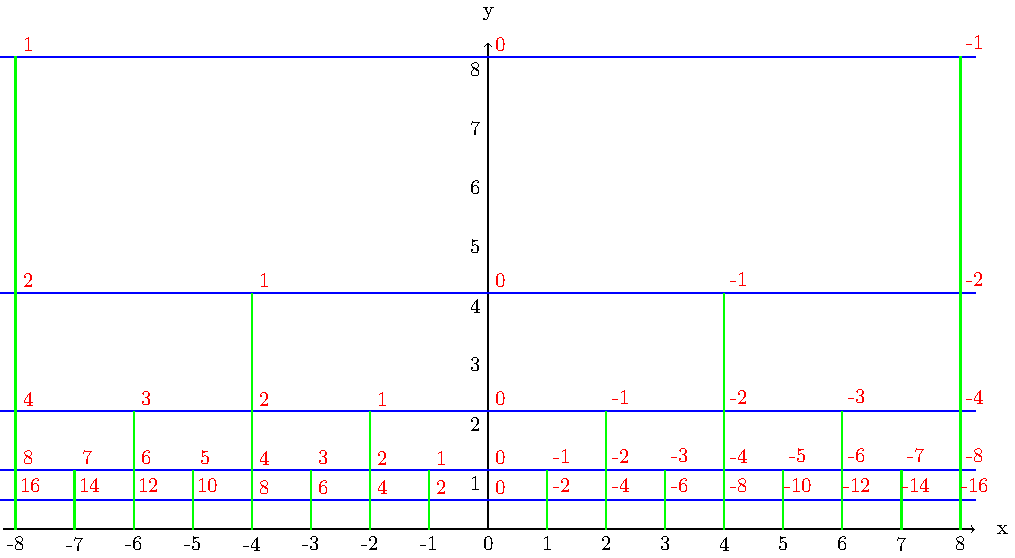
\includegraphics[width=0.8\textwidth]{figures/01-grid-example-1.pdf} 
        \caption{Conceptual example of a path in the (U,V) reference space. Specific paths from Table \ref{tab:knot41_data} would be plotted to analyze their geometric characteristics.}
        \label{fig:uv_path}
    \end{figure}
    \item **Role of $k_p, k_q, \sigma_{\text{eff}}$:** Understanding the precise relationship between the parameters $k_p, k_q, \sigma_{\text{eff}}$ (from the notes in Table \ref{tab:knot41_data}) and the derived integer $K$. These parameters likely encode information about how $p(a)$ and $q(a)$ are constructed from $\Delta(a)$ and cyclotomic factors, which in turn determines $K$.
\end{enumerate}

\section{Conclusion}
By directly analyzing the provided data for the $4_1$ knot, we have determined specific integer $K$ values associated with different relators. For the relator set including \texttt{aaBAbbbAB}, $K=-2$. For the set including \texttt{aBAABabbb}, $K=0$ (assuming $a$ is not a root of unity). This detailed analysis, incorporating the explicit data from `results.tex`, provides a concrete foundation for understanding the behavior of $K$ in the arithmetic torsion formula for the $4_1$ knot. Future work should focus on correlating these $K$ values with the algebraic and geometric properties of the paths.

\end{document}

